%!TEX root = ../main.tex
\documentclass{beamer} % Gliederung im Kopf, sections und subsections
\renewcommand{\baselinestretch}{1.2}\normalsize
\usetheme{default}
\setbeamertemplate{navigation symbols}{}
\setbeamertemplate{footline}[frame number]

\usepackage{tabu}
\usepackage{etex}
%\usepackage{beamerthemesplit}
%\useoutertheme[subsection=false]{smoothbars}
%\usepackage[final]{pdfpages}
\usepackage{bibentry}
\usepackage{bm}
\usepackage{bigints}
\usepackage{graphicx}
\usepackage{relsize}
\usepackage[round,longnamesfirst]{natbib}
\usepackage{bm}																									%matrix symbol
\usepackage{bbm}

\usepackage{paralist}

\usepackage{algpseudocode}
\usepackage{algorithmicx}
\usepackage{verbatim}
\usepackage{setspace}																					%Fu�noten (allgm.
\usepackage{hyperref}

\usepackage{bibentry}

\DeclareMathOperator*{\argmin}{arg\,min}
\DeclareMathOperator*{\argmax}{arg\,max}

\nobibliography*
\renewcommand{\vec}[1]{\mathbf{#1}}

\hypersetup{colorlinks=true,urlcolor=blue}														%Zeilenabst�nde)
\usepackage{threeparttable}
\usepackage{subfig}
\usepackage{epstopdf}
\usepackage{lscape}																							%Querformat
\usepackage[latin1]{inputenc}																		%Umlaute
\usepackage{graphicx}
\graphicspath{{../../material/}}

\usepackage{booktabs}
\usepackage{amsmath}
\usepackage{amssymb}
%\usepackage{uarial}

\usepackage{tabularx}
\usepackage{fancybox}																						%Boxen und Rahmen
\usepackage{appendix}
\usepackage{enumerate}

%EURO Symbol
\usepackage{tabularx}
\usepackage{longtable}																					%Mehrseitige Tabellen
\usepackage{fix-cm}
\usepackage[T1]{fontenc}
\usepackage{color,colortbl}																			%Farbige Tabellen
\usepackage{threeparttable}
\usepackage{hyperref}
\usepackage{amsfonts}

\usepackage{graphicx}
\usepackage{caption}

\usepackage{tikz}
\tikzset{
  treenode/.style = {shape=rectangle, rounded corners,
                     draw, align=center,
                     top color=white, bottom color=blue!20},
  root/.style     = {treenode, font=\Large, bottom color=red!30},
  env/.style      = {treenode, font=\ttfamily\normalsize},
  dummy/.style    = {circle,draw}
}
%\usepackage{cmbright}
\def\newblock{\hskip .11em plus .33em minus .07em}
\newcommand{\bs}{\boldsymbol}
\newcommand{\N}{\mathbb{N}}
\newcommand{\cov}{\mathrm{cov}\thin}
\newcommand{\thin}{\thinspace}
\newcommand{\thick}{\thickspace}

\newcommand{\vect}[1]{\mathbf{#1}}
\newcommand{\myfrac}[3][0pt]{\genfrac{}{}{}{}{\raisebox{#1}{$#2$}}{\raisebox{-#1}{$#3$}}}
\newcommand{\U}{\mathrm{U}}	%Uniform Distribution
\newcommand{\D}{\mathrm{D}}	%Dirichlet Distribution
\newcommand{\W}{\mathrm{W}}	%Wishart Distribution
\newcommand{\E}{\mathrm{E}}		%Expectation
\newcommand{\Prob}{\mbox{Pr}}		%Expectation
\newcommand{\Iden}{\mathbb{I}}	%Identity Matrix
\newcommand{\Ind}{\mathrm{I}}	%Indicator Function
\newcommand{\Tau}{\mathcal{T}\thin}

\newcommand{\var}{\mathrm{var}\thin}
\newcommand{\plim}{\mathrm{plim}\thin}
\newcommand\indep{\protect\mathpalette{\protect\independenT}{\perp}}
\def\independenT#1#2{\mathrel{\rlap{$#1#2$}\mkern5mu{#1#2}}}
\newcommand{\notindep}{\ensuremath{\perp\!\!\!\!\!\!\diagup\!\!\!\!\!\!\perp}}%

\newcommand{\mc}{\multicolumn}

\newcommand{\ph}{\phantom}
% weitere Optionen:
% secbar: Gliederung im Kopf, nur sections (alternativ zu subsecbar)
% handout: Produktion von Handouts, keine Animationen
\definecolor{darkblue}{rgb}{0,.35,.62}
\definecolor{lightblue}{rgb}{0.8,0.85,1}
\definecolor{lightgrey}{gray}{0.1}	%Farben mischen

%	kbordermatrix options

\makeatletter
\newcommand{\vast}{\bBigg@{4}}
\newcommand{\Vast}{\bBigg@{5}}
\makeatother
\newcommand{\indicator}[1]{\mathbbm{1}{\left\{ {#1} \right\} }}
\newcommand{\indic}{1{\hskip -2.5 pt}\hbox{1} }


\definecolor{lightgrey}{gray}{0.90}	%Farben mischen
\definecolor{grey}{gray}{0.85}
\definecolor{darkgrey}{gray}{0.65}
\definecolor{lightblue}{rgb}{0.8,0.85,1}

\renewcommand{\arraystretch}{1.5}


\usepackage{tikz}
\usetikzlibrary{trees,shapes,arrows,decorations.pathmorphing,backgrounds,positioning,fit,petri}
\renewcommand*{\familydefault}{\sfdefault}

\tikzset{forestyle/.style = {rectangle, thick, minimum width = 5cm, minimum height = 0.5cm, text width = 4.5cm, outer sep = 1mm},
	pre/.style={<-, shorten <=1pt, >=stealth, ultra thick},
	extend/.style={<-,dashed, shorten <=1pt, >=stealth, ultra thick}}
\captionsetup[subfigure]{labelformat=empty}


\newcommand{\beginbackup}{
   \newcounter{framenumbervorappendix}
   \setcounter{framenumbervorappendix}{\value{framenumber}}
}
\newcommand{\backupend}{
   \addtocounter{framenumbervorappendix}{-\value{framenumber}}
   \addtocounter{framenumber}{\value{framenumbervorappendix}}
}


% Begin Full Justification ---------------------------------------------------------

\usepackage{ragged2e}
% \usepackage{etoolbox}
\usepackage{lipsum}
\makeatletter
\renewcommand{\itemize}[1][]{%
  \beamer@ifempty{#1}{}{\def\beamer@defaultospec{#1}}%
  \ifnum \@itemdepth >2\relax\@toodeep\else
    \advance\@itemdepth\@ne
    \beamer@computepref\@itemdepth% sets \beameritemnestingprefix
    \usebeamerfont{itemize/enumerate \beameritemnestingprefix body}%
    \usebeamercolor[fg]{itemize/enumerate \beameritemnestingprefix body}%
    \usebeamertemplate{itemize/enumerate \beameritemnestingprefix body begin}%
    \list
      {\usebeamertemplate{itemize \beameritemnestingprefix item}}
      {\def\makelabel##1{%
          {%
            \hss\llap{{%
                \usebeamerfont*{itemize \beameritemnestingprefix item}%
                \usebeamercolor[fg]{itemize \beameritemnestingprefix item}##1}}%
          }%
        }%
      }
  \fi%
  \beamer@cramped%
  \justifying% NEW
  %\raggedright% ORIGINAL
  \beamer@firstlineitemizeunskip%
}

\justifying

% \apptocmd{\frame}{\justifying}{}{}

\usepackage{array}
\newcolumntype{L}[1]{>{\raggedright\let\newline\\\arraybackslash\hspace{0pt}}m{#1}}
\newcolumntype{C}[1]{>{\centering\let\newline\\\arraybackslash\hspace{0pt}}m{#1}}
\newcolumntype{R}[1]{>{\raggedleft\let\newline\\\arraybackslash\hspace{0pt}}m{#1}}



% End Full Justification ------------------------------------------------------------


\title{Parameters of Interest}
\author{Philipp Eisenhauer}

\date{}

\let\otp\titlepage
%\renewcommand{\titlepage}{\otp\addtocounter{framenumber}{-1}}

\begin{document}
\maketitle

\begin{frame}\begin{center}
\LARGE\textit{Housekeeping}
\end{center}\end{frame}

\begin{frame}
Since nearly all of you choose to review experimental studies. Please be sure to read ...

\begin{itemize}
\item \bibentry{Deaton.2009}
\item \bibentry{Imbens.2009}
\item \bibentry{Heckman.2009t}
\end{itemize}
\end{frame}

\begin{frame}
\begin{figure}\caption{Conditional Expectation and Essential Heterogeneity}
\scalebox{0.35}{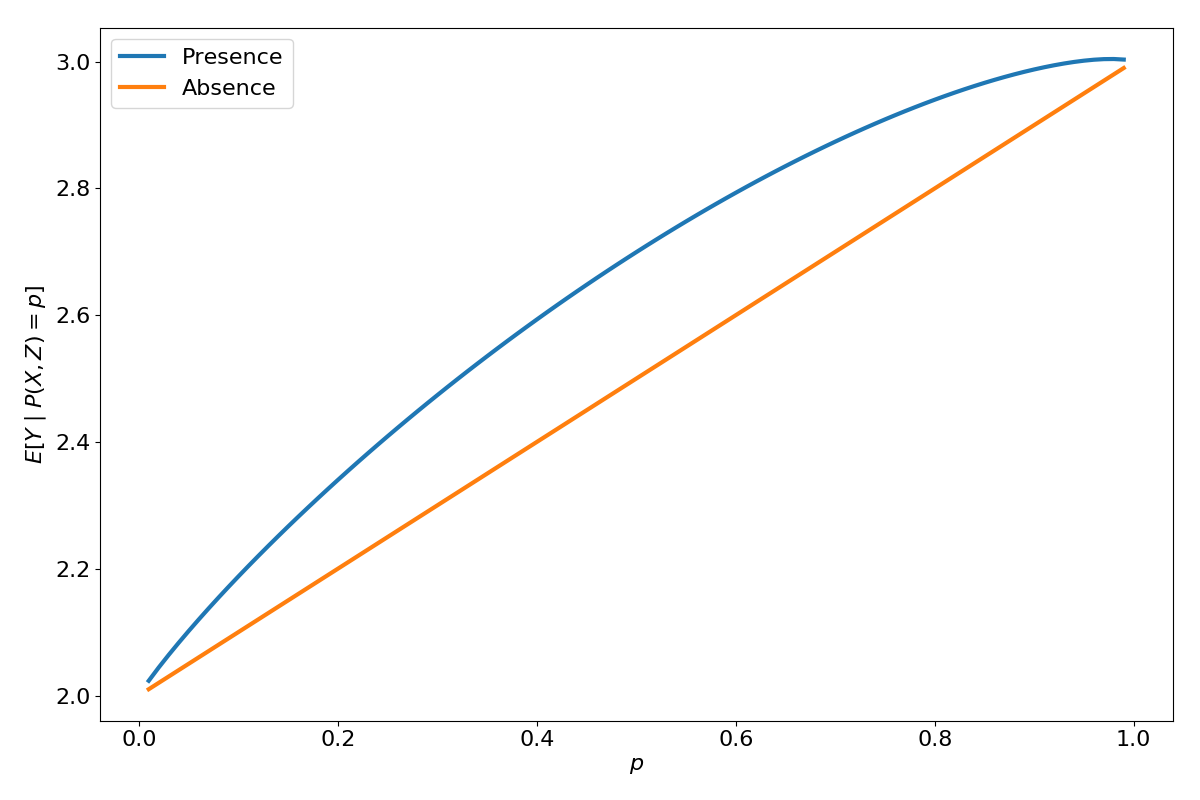
\includegraphics{fig-eh-conditional-expectation}}
\end{figure}
\end{frame}

\begin{frame}
\begin{figure}\caption{Marginal Treatment Effect and Essential Heterogeneity}
\scalebox{0.35}{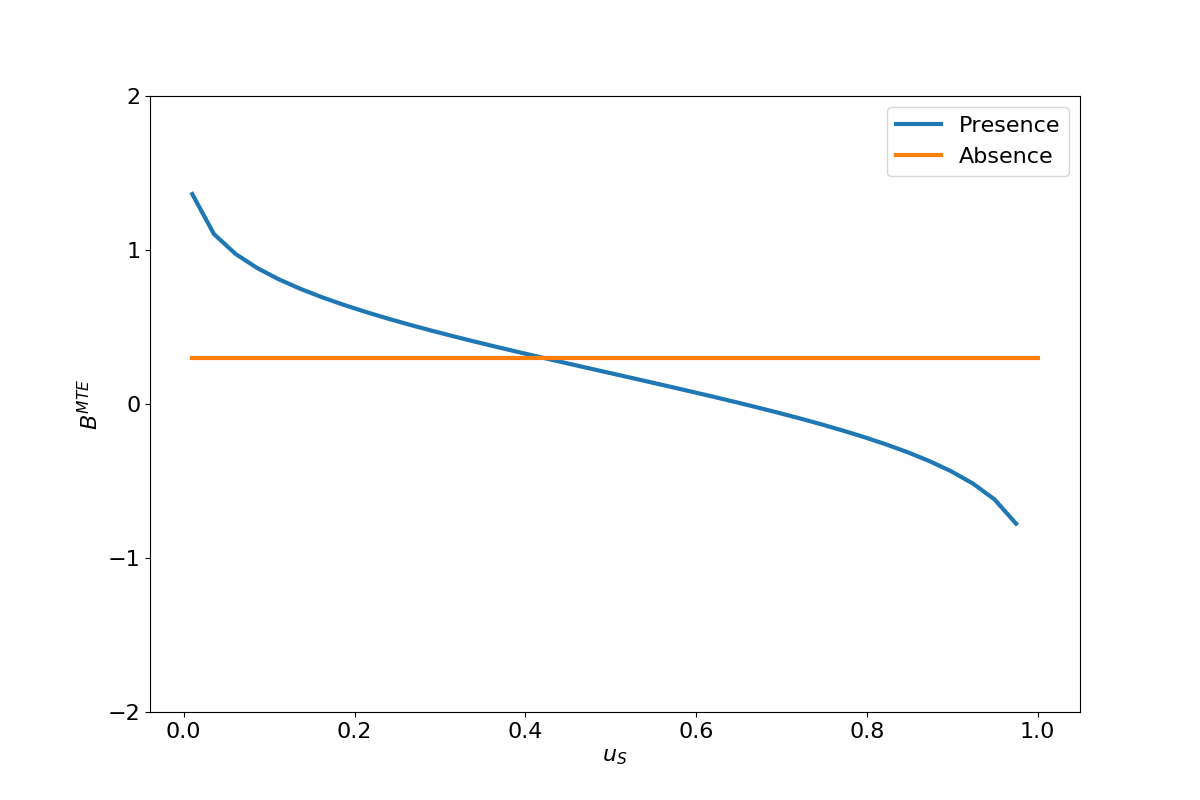
\includegraphics{fig-eh-marginal-effect}}
\end{figure}
\end{frame}

\begin{frame}
\begin{figure}\caption{Weights for Conventional Treatment Effect Parameters}
\scalebox{0.35}{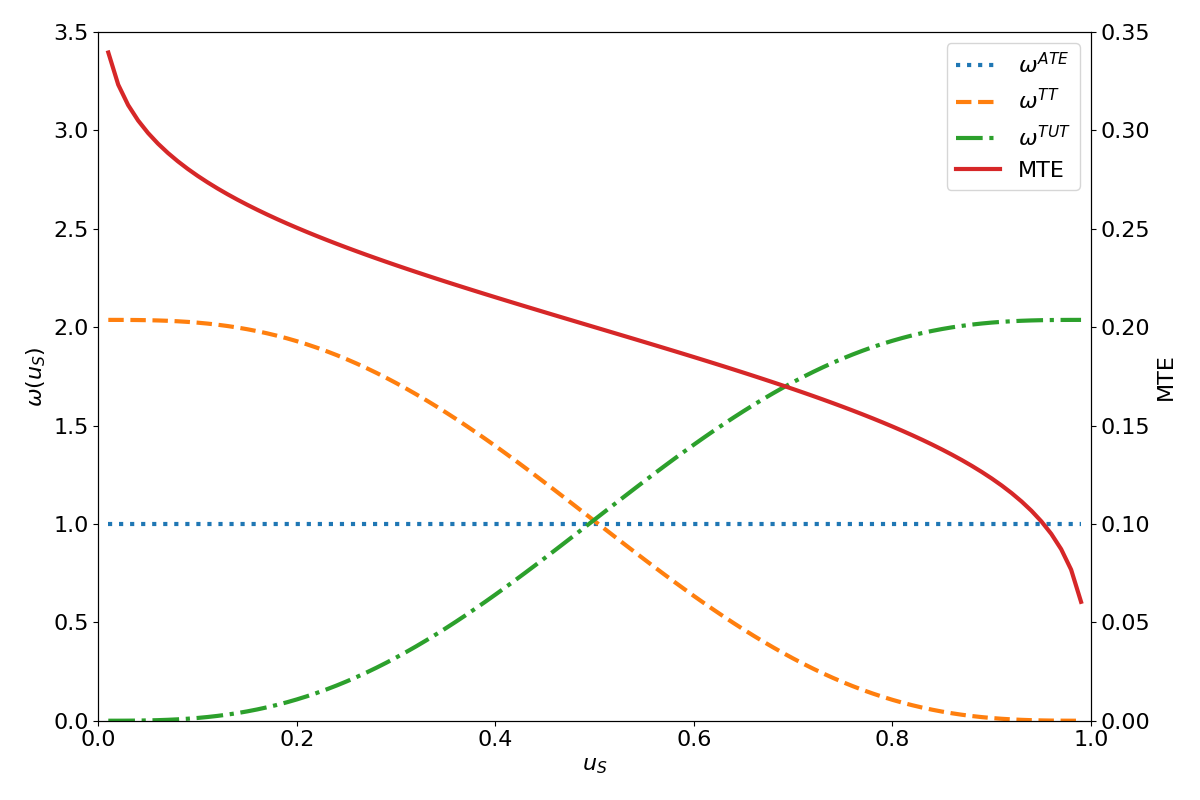
\includegraphics{fig-weights-marginal-effect}}
\end{figure}
\end{frame}


\begin{frame}
\begin{figure}\caption{Distribution of Conventional Effects}
\scalebox{0.35}{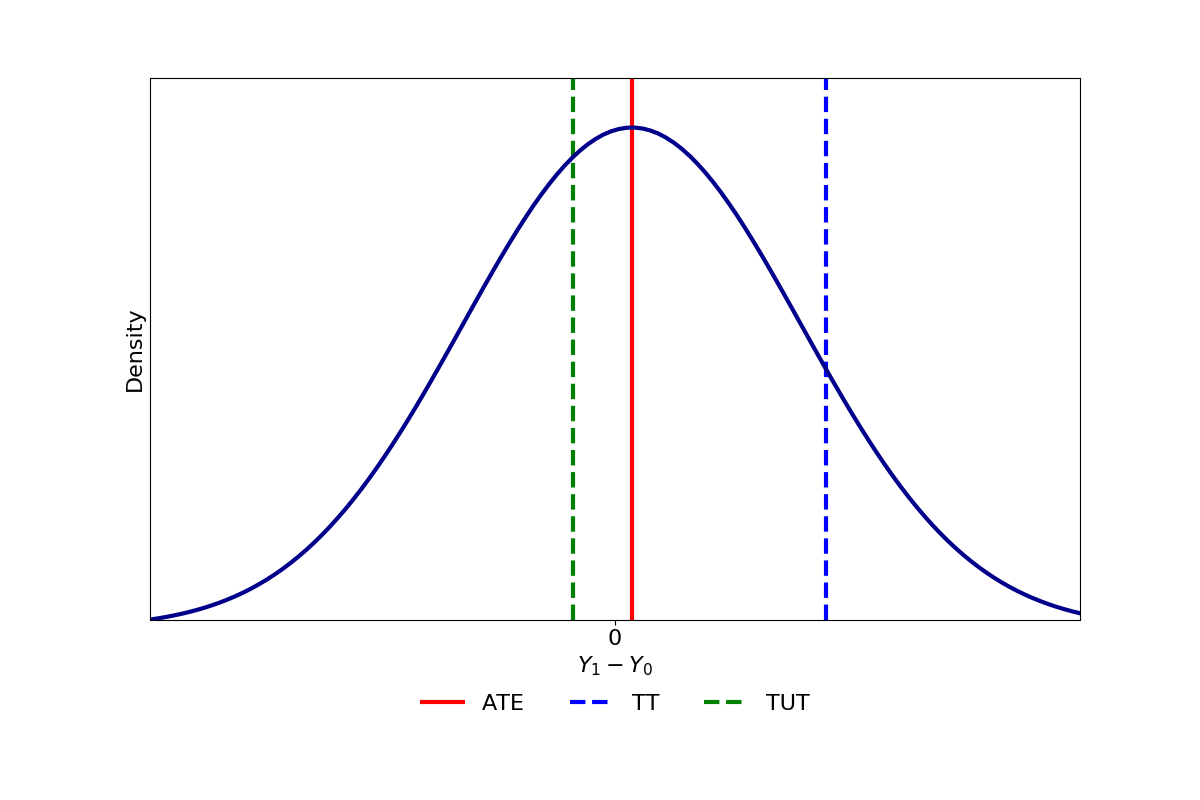
\includegraphics{fig-treatment-effects-conventional}}
\end{figure}
\end{frame}

\begin{frame}
\begin{figure}\caption{Distribution of Effects with Essential Heterogeneity}
\scalebox{0.35}{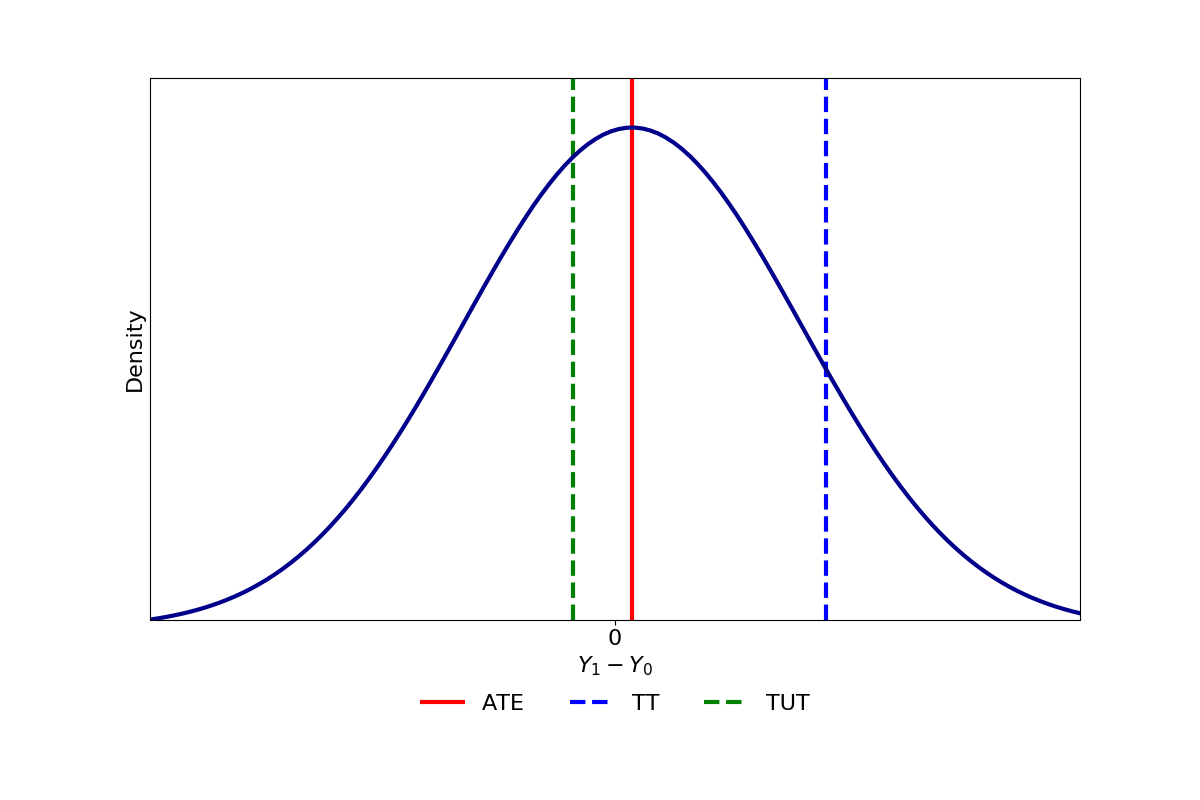
\includegraphics{fig-treatment-effects-with-eh}}
\end{figure}
\end{frame}


\begin{frame}
\begin{figure}\caption{Distribution of Effects without Essential Heterogeneity}
\scalebox{0.35}{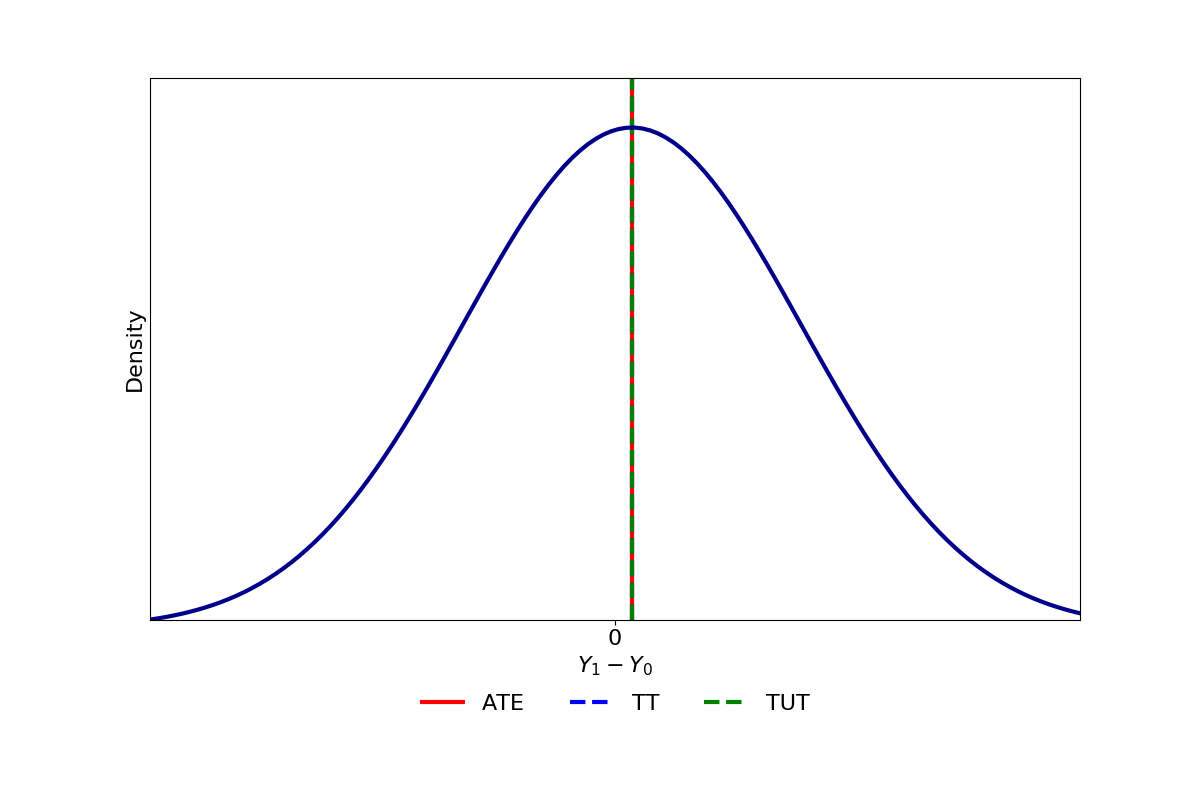
\includegraphics{fig-treatment-effects-without-eh}}
\end{figure}
\end{frame}

\begin{frame}
\begin{figure}\caption{Distribution of Benefits}
\scalebox{0.35}{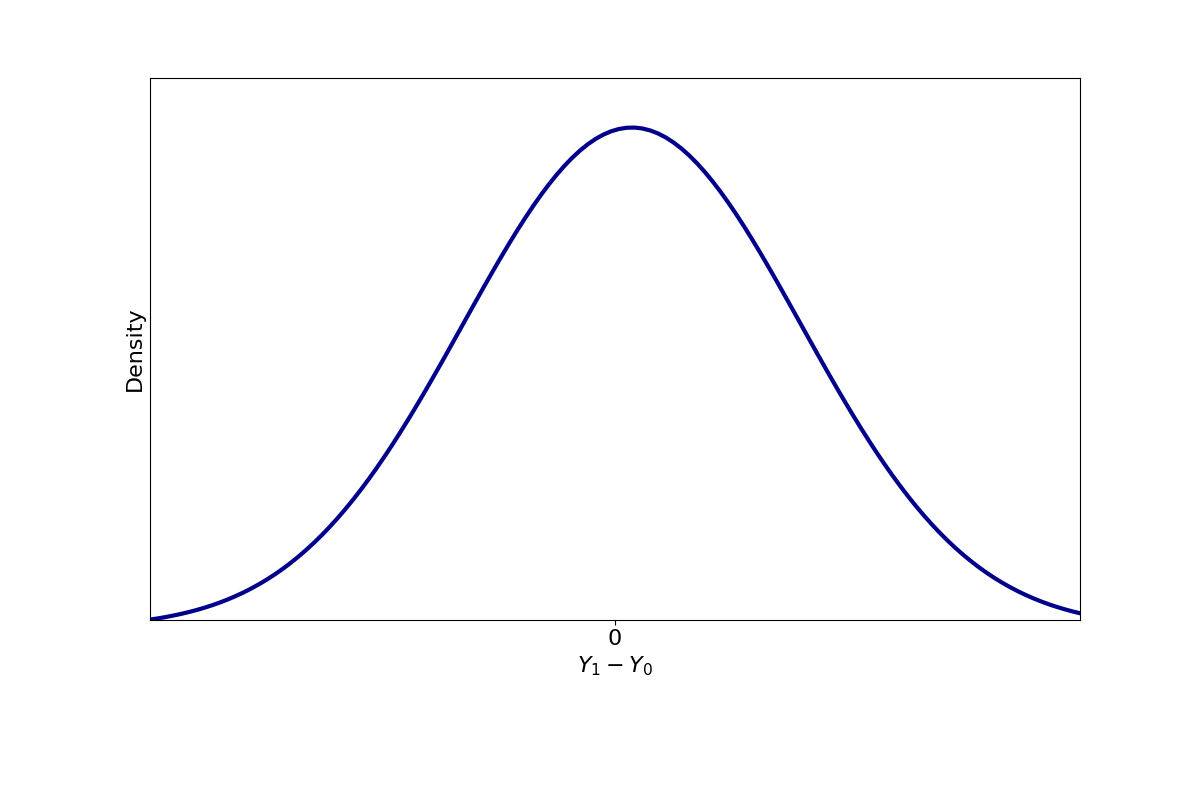
\includegraphics{fig-treatment-effects-benefits}}
\end{figure}
\end{frame}

\begin{frame}
\begin{figure}\caption{Distribution of Benefits by Treatment Status}
\scalebox{0.35}{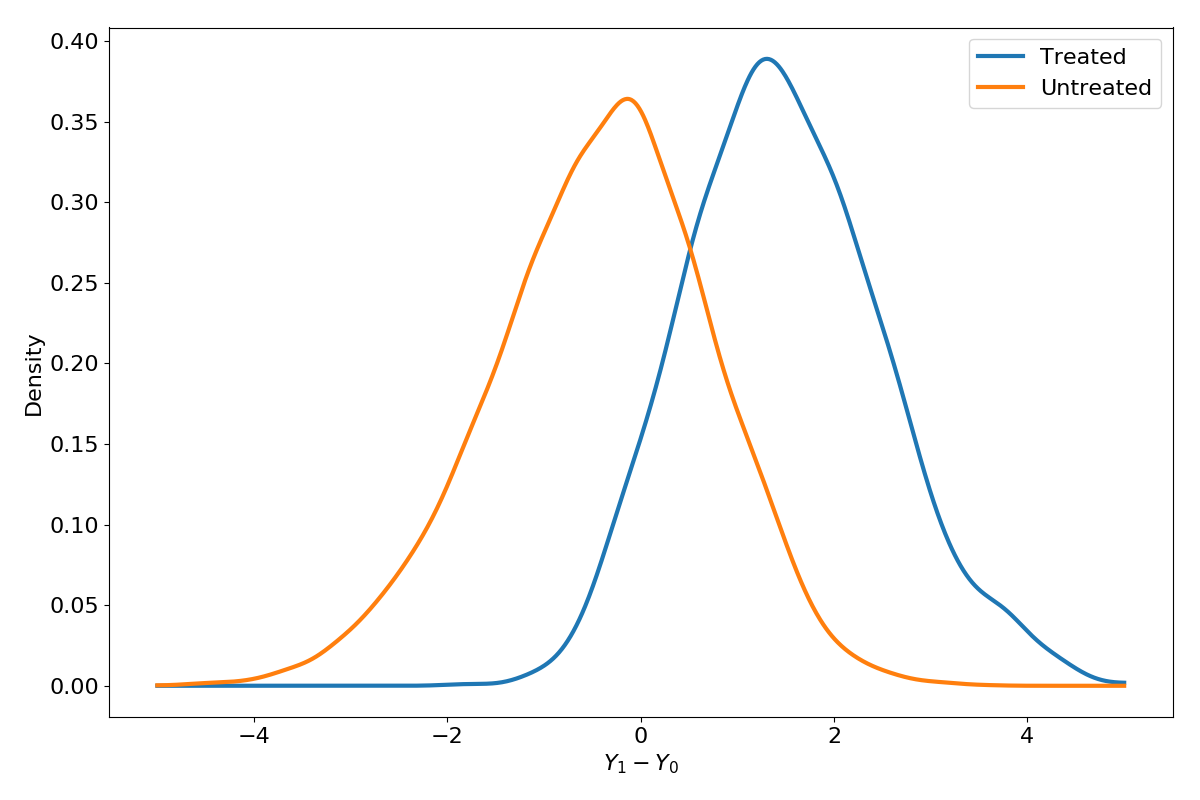
\includegraphics{fig-treatment-effects-treatment}}
\end{figure}
\end{frame}

\begin{frame}
\begin{figure}\caption{Distribution of Benefits by Policy}
\scalebox{0.35}{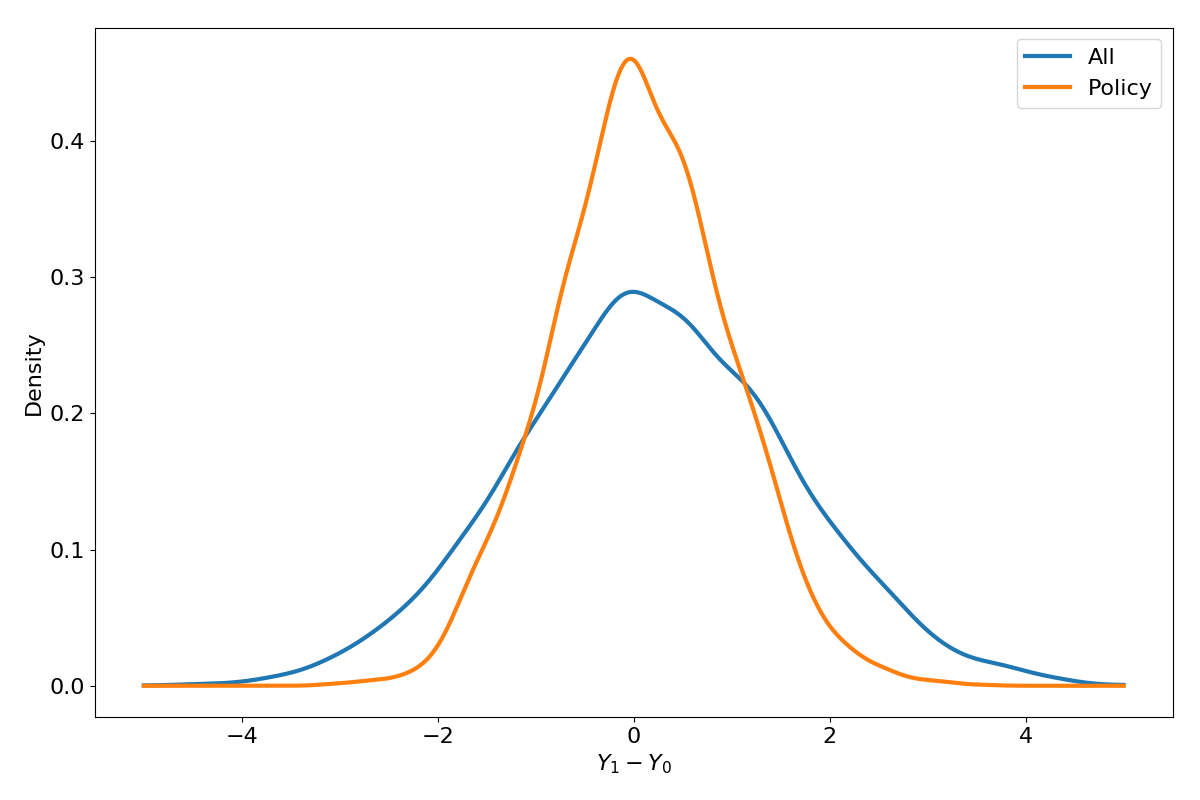
\includegraphics{fig-treatment-effects-policy}}
\end{figure}
\end{frame}

\begin{frame}
\begin{figure}\caption{Distribution of Potential Outcomes}
\scalebox{0.35}{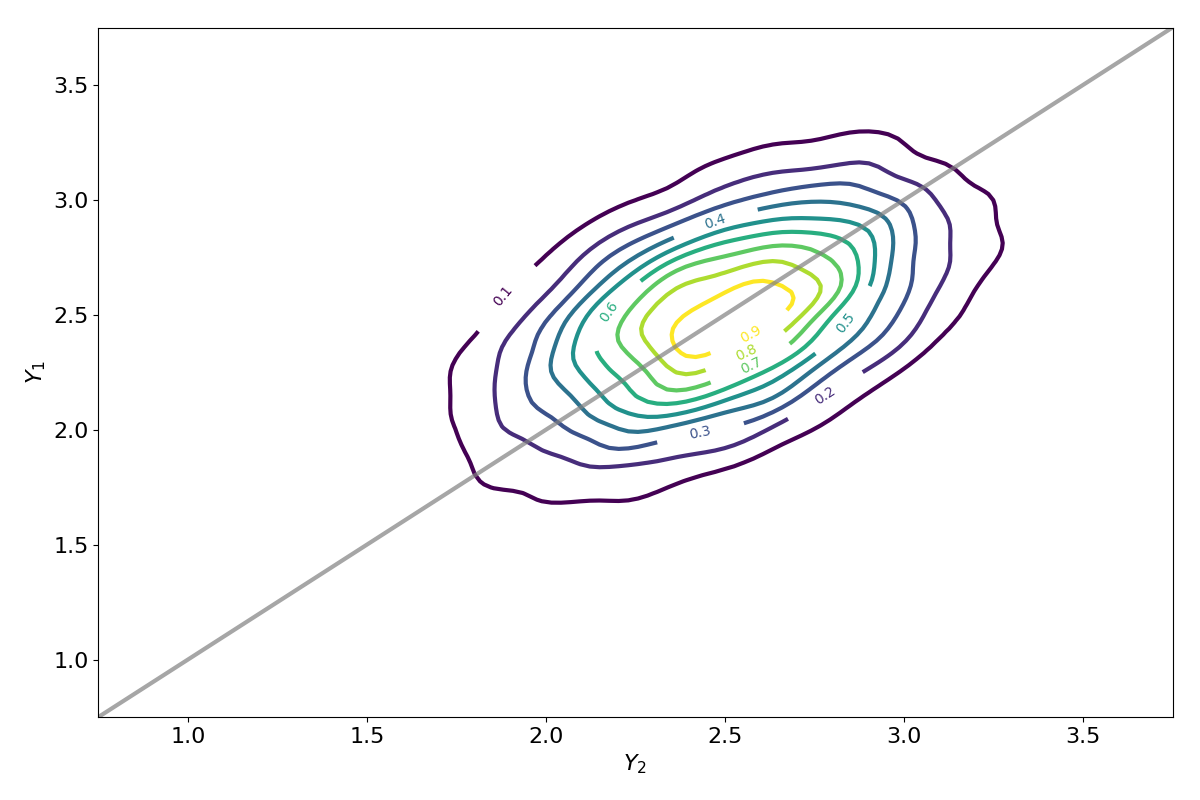
\includegraphics{fig-distribution-potential}}
\end{figure}
\end{frame}

\begin{frame}
\begin{figure}\caption{Distribution of Benefits and Surplus}
\scalebox{0.35}{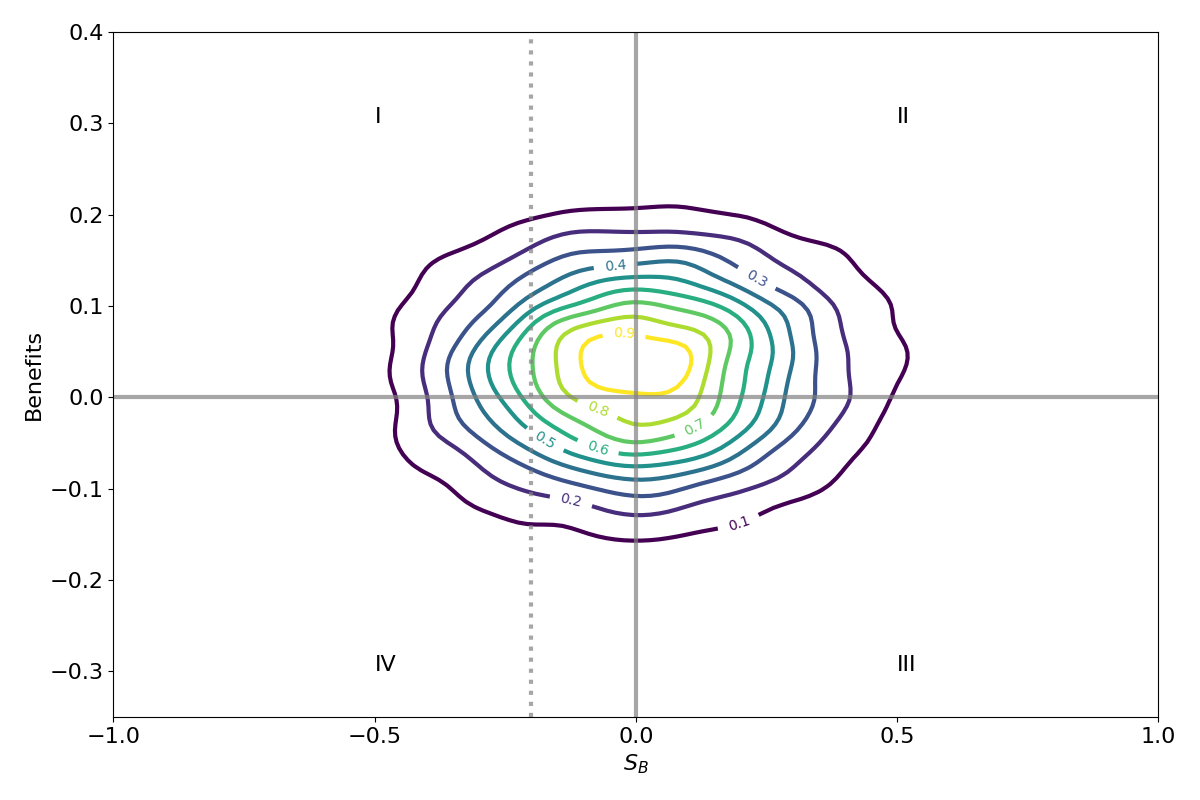
\includegraphics{fig-distribution-surplus}}
\end{figure}
\end{frame}

\begin{frame}
\begin{figure}\caption{Margin of Indifference}
\scalebox{0.35}{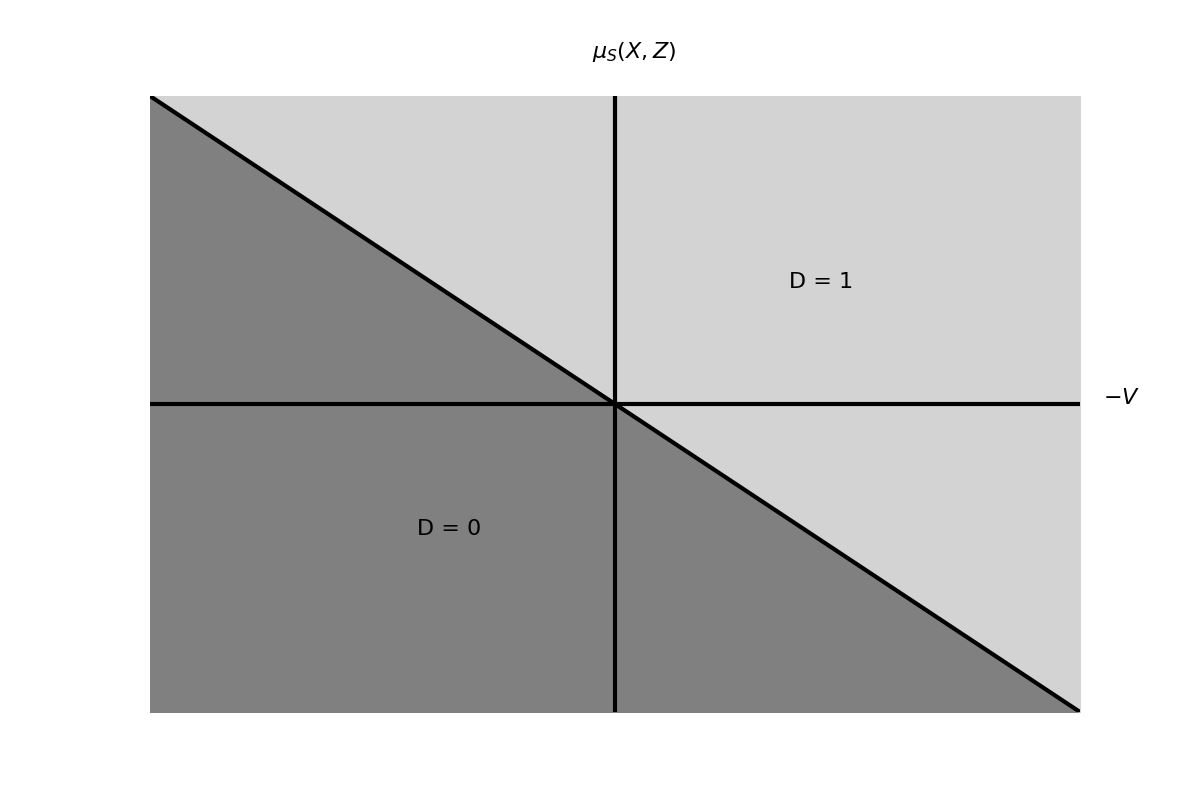
\includegraphics{fig-margin-indifference}}
\end{figure}
\end{frame}

\begin{frame}
\begin{figure}\caption{Local Average Treatment Effect}
\scalebox{0.35}{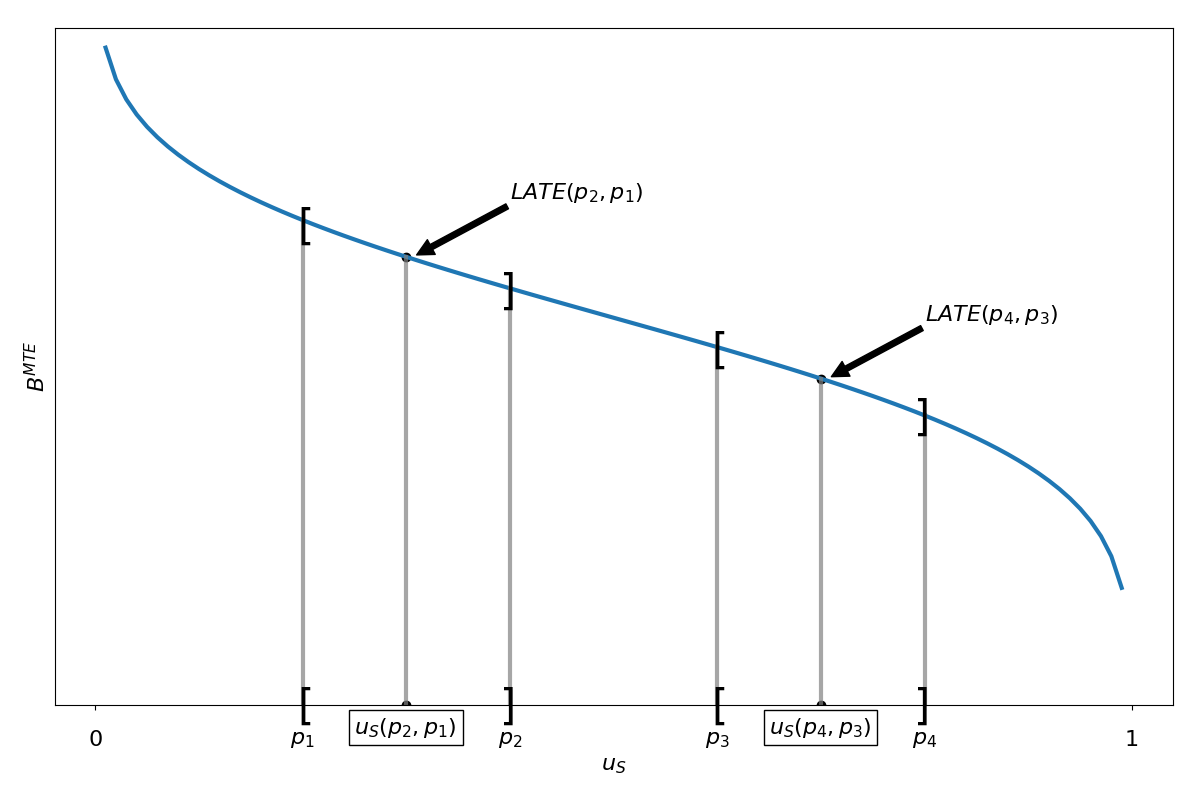
\includegraphics{fig-local-average-treatment}}
\end{figure}
\end{frame}

\beginbackup\appendix
\begin{frame}\begin{center}
\LARGE\textbf{Appendix}
\end{center}\end{frame}

%------------------------------------------------------------------------------
%------------------------------------------------------------------------------
\begin{frame}\begin{center}
\LARGE\textit{References}
\end{center}\end{frame}
%------------------------------------------------------------------------------
%------------------------------------------------------------------------------
\newgeometry{margin=1cm}
\begin{frame}[allowframebreaks]\frametitle{}

\nocite{Carneiro.2011, Heckman.1990c, Heckman.2010h}

\bibliographystyle{apalike}
\bibliography{../../../submodules/bibliography/literature}


\end{frame}

\backupend
\end{document}
